% ============================================================
%  SmartDoc AI — IEEE Conference Paper
%  Open Source Software Development Course, Spring 2026
%  Saigon University (Đại học Sài Gòn)
%
%  Compile with: pdflatex smartdoc-ai-ieee-report.tex
%               bibtex  smartdoc-ai-ieee-report
%               pdflatex smartdoc-ai-ieee-report.tex  (twice)
% ============================================================

\documentclass[10pt, conference, a4paper, compsocconf]{IEEEtran}

\usepackage{amsmath,amsxtra,amssymb,amsthm,latexsym,amscd,amsfonts}
\usepackage[english]{babel}
% \usepackage[utf8]{vietnam}
\usepackage[top=2.7cm, bottom=5.4cm, left=2.72cm, right=3.0cm]{geometry}
\headsep=0.7cm
\headheight=1.0cm
\footskip=1.0cm
\voffset=-0.74cm

\usepackage{fancyhdr}
\pagestyle{fancy}
\renewcommand{\sectionmark}[1]{\markright{\MakeUppercase{#1}}{}}
\renewcommand{\headrulewidth}{0pt}

\ifCLASSINFOpdf
  \usepackage[pdftex]{graphicx}
  \usepackage{pgfplots}
  \pgfplotsset{compat=1.17}
  \DeclareGraphicsExtensions{.pdf,.jpeg,.png,.jpg}
\else
  \usepackage[dvips]{graphicx}
  \DeclareGraphicsExtensions{.eps}
\fi

\usepackage{tikz}
\usetikzlibrary{shapes.geometric, arrows.meta, positioning, fit, backgrounds}

\usepackage{array}
\usepackage[hyphens]{url}  % allow line breaks in URLs at hyphens
\usepackage{float}
\usepackage{booktabs}
\usepackage{microtype}   % character protrusion & font expansion to reduce overfull boxes
\usepackage[caption=false,font=footnotesize]{subfig}

\makeatletter
\def\ps@IEEEtitlepagestyle{%
  \def\@oddhead{\centering{\mbox{\footnotesize{\textit{%
    \;\;\;\; Major Project: Open Source Software Development Course
    -- Saigon University, April 22, 2026}}}}}%
  \def\@evenhead{\centering{\mbox{\footnotesize{\textit{%
    \;\;\;\; Major Project: Open Source Software Development Course
    -- Saigon University, April 22, 2026}}}}}%
  \def\@oddfoot{\scriptsize \thepage \hfil }%
  \def\@evenfoot{\scriptsize \hfil \thepage}
}
\makeatother

% ============================================================

\begin{document}
\pagenumbering{arabic}
\fontsize{10}{12}
\selectfont
% Allow slightly loose word spacing to prevent overfull hboxes (long monospace strings, URLs)
\sloppy
\setlength{\emergencystretch}{3em}

\fancyhead[RE,LO]{\centering{\footnotesize{\textit{%
  Major Project: Open Source Software Development Course
    -- Saigon University, April 22, 2026}}}}

% ============================================================
%  Title and Authors
% ============================================================

\title{SmartDoc AI: A Privacy-First Local Document Intelligence System
       with Dual-Pipeline Retrieval-Augmented Generation}

\author{
  \IEEEauthorblockN{%
    Tran Quang Dung\IEEEauthorrefmark{1},
    Tran Thi Tinh\IEEEauthorrefmark{2},
    Le Quoc Cuong\IEEEauthorrefmark{3},
    Le Tien Đuc\IEEEauthorrefmark{4},
    Hoang Quoc Cuong\IEEEauthorrefmark{5}}
  \IEEEauthorblockA{%
    Faculty Of Information Technology, Saigon University}
  \IEEEauthorblockA{%
    \IEEEauthorrefmark{1}dungtranquang2005@gmail.com,
    \IEEEauthorrefmark{2}tinhtt.sgu@gmail.com,
    \IEEEauthorrefmark{3}lequoccuong2204@gmail.com\\
    \IEEEauthorrefmark{4}ltd9605@gmail.com,
    \IEEEauthorrefmark{5}cuongsc2411@gmail.com}
}

\maketitle

% ============================================================
%  Abstract
% ============================================================

\begin{abstract}
Large language models (LLMs) offer powerful text-generation capabilities,
but frequently produce hallucinated or ungrounded answers when applied to
domain-specific documents. Retrieval-Augmented Generation (RAG) mitigates
this by grounding responses in retrieved evidence; however, a standard
single-pass RAG pipeline can still fail silently when initial retrieval
yields insufficient context. This paper presents \emph{SmartDoc AI}, an
open-source, privacy-first document intelligence system inspired by Google's
NotebookLM. Running entirely on local infrastructure via Ollama
(Qwen2.5:7b) and FAISS, the system ensures that user documents never leave
the local machine. Its core contribution is a \emph{dual-pipeline
architecture} that runs Self-RAG and Co-RAG independently on every query
and displays both results side-by-side for comparison. Self-RAG implements
multi-hop retrieval with quality-gated candidate scoring and an automated
repair agent, while Co-RAG employs an iterative Generator--Reviewer
collaboration loop. Both pipelines share a hybrid search engine combining
dense semantic retrieval and sparse BM25 keyword matching via Reciprocal
Rank Fusion, followed by Cross-Encoder reranking. Experimental evaluation
demonstrates that both pipelines substantially improve groundedness,
utility, and relevance compared to a single-pass RAG baseline.
\end{abstract}

\begin{IEEEkeywords}
retrieval-augmented generation; Self-RAG; Co-RAG; hybrid search;
FAISS; Ollama; document intelligence; local LLM; open-source
\end{IEEEkeywords}

\IEEEpeerreviewmaketitle

% ============================================================
%  Section I — Introduction
% ============================================================

\section{Introduction}

The rapid advancement of large language models has generated significant
interest in intelligent document question-answering systems. Cloud-based
services such as Google's NotebookLM~\cite{notebooklm} offer document-grounded
chat capabilities but require users to upload sensitive documents to
third-party servers, raising privacy, data-sovereignty, and compliance
concerns. Local alternatives often provide only rudimentary single-pass
RAG pipelines without quality validation, leaving users uncertain about
answer reliability.

Retrieval-Augmented Generation (RAG)~\cite{rag_lewis2020} addresses LLM
hallucination by combining a dense retriever with a generative model.
Nevertheless, standard RAG pipelines are vulnerable to silent failure:
if the first retrieval pass returns irrelevant or sparse context, the
generator produces low-quality responses without any warning signal.

SmartDoc AI addresses these limitations with the following contributions:

\begin{itemize}
  \item A fully \emph{local, privacy-preserving architecture} powered by
        Ollama~\cite{ollama} and FAISS~\cite{faiss} requiring no cloud
        connectivity or API keys.

  \item A \emph{dual-pipeline RAG design} that runs Self-RAG~\cite{selfrag_asai2023}
        and Co-RAG~\cite{corag_jin2025} independently on every query,
        providing complementary reasoning strategies and enabling
        direct side-by-side quality comparison.

  \item A \emph{hybrid search engine} that fuses dense semantic retrieval
        and sparse BM25 keyword matching via Reciprocal Rank Fusion
        (RRF)~\cite{hybrid_search}, followed by Cross-Encoder reranking.

  \item A \emph{Markdown-aware document ingestion pipeline} that converts
        PDF and DOCX files into structure-preserving Markdown, improving
        chunk coherence and heading-context retention.

  \item A \emph{per-notebook configuration system} that allows users to
        customize retrieval depth, quality thresholds, and LLM temperature
        independently for each notebook through the Streamlit UI.
\end{itemize}

% ============================================================
%  Section II — Related Work
% ============================================================

\section{Related Work}

\subsection{Retrieval-Augmented Generation}
Lewis et al.~\cite{rag_lewis2020} introduced RAG as a method for
knowledge-intensive NLP tasks by combining a non-parametric dense retriever
with a sequence-to-sequence generator. The retriever fetches relevant
document passages that are concatenated with the query and passed to the
generator, significantly reducing hallucination. Subsequent work has
explored a variety of retrieval strategies, including Dense Passage
Retrieval (DPR), BM25 hybrid fusion, and multi-hop reasoning
chains~\cite{hybrid_search}.

\subsection{Self-RAG}
Asai et al.~\cite{selfrag_asai2023} proposed Self-RAG, which trains a
single model to insert special reflection tokens---\textsc{isrel},
\textsc{issup}, and \textsc{isuse}---to decide adaptively when to retrieve,
to evaluate passage relevance, and to critique its own output.
SmartDoc AI adapts this concept by using a separate LLM judge to score
independently generated candidate answers against the same three criteria,
eliminating the requirement for a specially fine-tuned model and making the
approach accessible with any instruction-tuned LLM.

\subsection{Collaborative Multi-Agent Generation}
The Co-RAG pipeline in SmartDoc AI is inspired by multi-agent
collaboration frameworks~\cite{corag_jin2025}, in which a Generator and a
Reviewer engage in iterative critique-and-refine cycles. The Reviewer
explicitly diagnoses hallucinations, factual gaps, and reasoning errors in
the Generator's draft and produces targeted corrective feedback that the
Generator applies in subsequent iterations.

\subsection{Local LLM Inference and Open-Source Tools}
Ollama~\cite{ollama} provides a lightweight server for running quantized
open-source LLMs locally. Combined with the Qwen2.5:7b model~\cite{qwen25},
which demonstrates strong multilingual reasoning capabilities in both
English and Vietnamese, SmartDoc AI achieves competitive answer quality
without cloud API dependencies. The system also relies on
LangChain~\cite{langchain} for pipeline orchestration and prompt
management, and on Sentence Transformers~\cite{reimers2019} for
multilingual document embeddings.

% ============================================================
%  Section III — System Architecture
% ============================================================

\section{System Architecture}

\subsection{Overview}

SmartDoc AI consists of two decoupled pipelines: an \emph{Ingestion
Pipeline} that converts uploaded documents into searchable FAISS vector
indices, and a \emph{Query Pipeline} that processes user questions through
the dual-RAG strategy. All tunable parameters (retrieval depth, quality
thresholds, model names, chunk sizes) are centralized in
\texttt{core/configs.py}, enabling per-notebook customization without
code changes. Figure~\ref{fig:arch} illustrates the high-level architecture.

\begin{figure}[H]
\centering
\resizebox{\linewidth}{!}{%
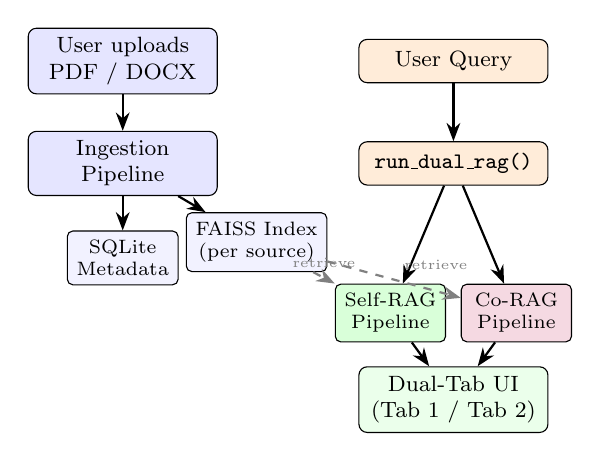
\begin{tikzpicture}[
  >=Stealth,
  block/.style={
    draw, rectangle, rounded corners=3pt,
    minimum width=2.4cm, minimum height=0.55cm,
    align=center, font=\footnotesize, fill=white
  },
  smallblock/.style={
    draw, rectangle, rounded corners=2pt,
    minimum width=1.4cm, minimum height=0.48cm,
    align=center, font=\scriptsize, fill=white
  },
  arrow/.style={->, thick}
]

% --- Ingestion side ---
\node[block, fill=blue!10]  (upload) at (-2.2, 4.5) {User uploads\\PDF / DOCX};
\node[block, fill=blue!10]  (ingest) at (-2.2, 3.2) {Ingestion\\Pipeline};
% SQLite stays below ingest (straight down arrow)
\node[smallblock, fill=blue!5]  (sqlite) at (-2.2, 2.0) {SQLite\\Metadata};
% FAISS repositioned to center-left so both retrieve arrows are short diagonals
% that pass ABOVE selfrag/corag nodes — no crossings
\node[smallblock, fill=blue!5]  (faiss)  at (-0.5, 2.2) {FAISS Index\\(per source)};

\draw[arrow] (upload) -- (ingest);
\draw[arrow] (ingest) -- (sqlite);
\draw[arrow] (ingest) -- (faiss);

% --- Query side ---
\node[block, fill=orange!15] (query)   at (2.0, 4.5) {User Query};
\node[block, fill=orange!15] (orch)    at (2.0, 3.2) {\texttt{run\_dual\_rag()}};
\node[smallblock, fill=green!15]  (selfrag) at (1.2, 1.3) {Self-RAG\\Pipeline};
\node[smallblock, fill=purple!15] (corag)   at (2.8, 1.3) {Co-RAG\\Pipeline};
\node[block, fill=green!8]   (ui)      at (2.0, 0.2) {Dual-Tab UI\\(Tab 1 / Tab 2)};

\draw[arrow] (query)   -- (orch);
\draw[arrow] (orch)    -- (selfrag);
\draw[arrow] (orch)    -- (corag);
\draw[arrow] (selfrag) -- (ui);
\draw[arrow] (corag)   -- (ui);

% --- FAISS feeds BOTH pipelines via short diagonal arrows ---
% faiss(-0.5,2.2)→selfrag(1.2,1.3): short diagonal, clear
% faiss(-0.5,2.2)→corag(2.8,1.3): longer diagonal, but at x=1.2 it is at y≈1.74
%   which is above selfrag top edge (y≈1.54) — no crossing
\draw[arrow, dashed, gray] (faiss) --
  node[above, font=\tiny]{retrieve} (selfrag);
\draw[arrow, dashed, gray] (faiss) --
  node[above right, font=\tiny]{retrieve} (corag);

\end{tikzpicture}%
}% end \resizebox
\caption{High-level architecture of SmartDoc AI. The Ingestion Pipeline
(left) populates per-source FAISS indices and SQLite metadata. The Query
Pipeline (right) runs Self-RAG and Co-RAG in parallel and displays results
in a dual-tab Streamlit UI.}
\label{fig:arch}
\end{figure}

\subsection{Document Ingestion Pipeline}

The ingestion pipeline transforms raw documents into per-source FAISS
vector indices through five sequential stages.

\textbf{(1) File-type detection.} File type is determined by reading
raw magic bytes: \texttt{\%PDF} identifies PDFs; the \texttt{PK} ZIP
signature identifies DOCX files. Unsupported formats are rejected before
any further processing.

\textbf{(2) Duplicate detection.} An MD5 hash of the raw file bytes is
computed prior to processing. If a source with the same hash already exists
within the same notebook, the upload is silently skipped, preventing
duplicate indices and redundant computation.

\textbf{(3) Markdown conversion.} PDFs are converted using
PyMuPDF's \texttt{page.get\_text("dict")} interface. Per-page font-size
statistics are collected; the median body-text font size is used as a
baseline to infer heading levels (\texttt{\#}, \texttt{\#\#}, \texttt{\#\#\#}).
Span flags decode bold (bit~4) and italic (bit~1) to Markdown markup.
DOCX files are walked element-by-element over \texttt{w:p} (paragraphs)
and \texttt{w:tbl} (tables) XML nodes to produce Markdown headings,
bullet lists, and pipe tables, preserving the original document structure.

\textbf{(4) Markdown-aware chunking.} A
\texttt{MarkdownHeaderTextSplitter} first divides the document at
\texttt{\#}--\texttt{\#\#\#\#} headers, retaining header context inside
each chunk. Sections exceeding \texttt{rag\_max\_chunk\_len} characters
are further subdivided by \texttt{RecursiveCharacterTextSplitter} with
configurable chunk overlap.

\textbf{(5) Embedding and storage.} Chunks are embedded with the
\texttt{paraphrase-multilingual-mpnet-base-v2}
model (768-dimensional vectors, multilingual support)
using GPU acceleration with automatic CPU fallback. Each source receives an isolated FAISS \texttt{IndexFlatL2}
index stored at the path
\texttt{vectorstores/\{notebook\_id\}/\{source\_id\}/}. Per-source
isolation enables selective retrieval and clean deletion without affecting
other documents in the same notebook.

\subsection{Hybrid Search Engine}

The search engine supports three retrieval modes selected by the
configurable weight parameters \texttt{weight\_semantic} ($\alpha_s$)
and \texttt{weight\_bm25} ($\alpha_b$).

\textbf{Pure Semantic Search ($\alpha_b = 0$):} FAISS L2-distance
similarity search returns the top-$k$ chunks, filtered by a configurable
score threshold.

\textbf{Pure BM25 Search ($\alpha_s = 0$):} Sparse keyword matching
followed by cross-validation against semantic similarity scores to allow
meaningful threshold filtering.

\textbf{Hybrid Search (both $> 0$):} Semantic and BM25 results are fused
via Reciprocal Rank Fusion (RRF). For each candidate document~$d$, the
combined score is:
\begin{equation}
  \text{RRF}(d) = \sum_{r \in R} \frac{1}{c + \text{rank}_r(d)},
  \label{eq:rrf}
\end{equation}
where $R$ is the set of rank lists, $\text{rank}_r(d)$ is the position of
$d$ in list~$r$, and $c = 60$ is the smoothing constant. The allocation of
retrieved documents between semantic and BM25 is proportional to the
configured weights; e.g., with \texttt{top\_n}~$= 16$ and equal weights,
each retriever contributes 8 candidates.

After pooling, if the candidate count is at least
\texttt{rag\_final\_context\_k}, Cross-Encoder reranking is applied.
Every (query, chunk) pair is scored by the
\texttt{cross-encoder/ms-marco-MiniLM-L-6-v2} model; the top-$k$ chunks
are selected for the generator. Deduplication by document identifier
is applied before reranking to remove overlapping results produced by
the semantic and BM25 retrievers.

\subsection{Self-RAG Pipeline}

The Self-RAG pipeline~\cite{selfrag_asai2023} implements a multi-hop,
quality-gated retrieval loop with automatic repair.

\textbf{Step~0 — Intent routing.} A two-layer greeting detector
classifies the reformulated query. Layer~1 applies a multilingual regex
lookup; Layer~2 calls the LLM classifier for ambiguous inputs. Greeting
queries are handled directly by the LLM; factual queries proceed to Step~1.

\textbf{Step~1 — Search plan generation.} An LLM decomposes the
reformulated query into 1--3 independent sub-queries, each targeting a
distinct search angle. After a repair cycle, the repair agent's revised
sub-queries replace the previous failed plan.

\textbf{Step~2 — Multi-hop retrieval.} For each sub-query, the hybrid
search engine is invoked. Sub-queries returning zero results are rewritten
by the LLM and retried up to \texttt{self\_rag\_max\_retries\_per\_hop}
times. Retrieved chunks are deduplicated by content hash, merged into a
shared pool, and reranked by Cross-Encoder.

\textbf{Step~3 — Candidate generation.} The LLM generates
\texttt{self\_rag\_candidates} diverse answer drafts using temperatures
spread around \texttt{llm\_avg\_temp}, encouraging coverage of different
phrasings and reasoning paths.

\textbf{Step~4 — Quality scoring and winner selection.} An LLM judge
evaluates each candidate on two dimensions: ISSUP (groundedness—is the
answer supported by retrieved context?) and ISUSE (utility—does the
answer satisfy user intent?). ISREL (relevance) is derived from the
mean sigmoid-normalized Cross-Encoder scores of the reranked context.
The final confidence score is:
\begin{equation}
  \text{conf} = 0.25 \cdot \text{ISREL}
              + 0.50 \cdot \text{ISSUP}
              + 0.25 \cdot \text{ISUSE}.
  \label{eq:conf}
\end{equation}
The winner is selected by highest confidence score, with tie-breaking in
priority order: answer status (\textsc{doc\_answer} $\succ$
\textsc{doc\_general} $\succ$ \textsc{doc\_missing}), then ISSUP score,
then generation index.

\textbf{Step~5a — Quality gate.} If all three scores meet the configured
thresholds ($\geq$ \texttt{threshold\_issup/isrel/isuse}), the winner is
returned with its confidence score and reasoning trace.

\textbf{Step~5b — Repair agent.} If any threshold is not met and
\texttt{self\_rag\_max\_depth} has not been exhausted, a repair agent
diagnoses which gates failed, identifies the root cause, and generates a
new search plan targeting different angles. An oscillation guard prevents
repeating an identical search plan. The pipeline restarts from Step~1
with depth incremented by one.

\subsection{Co-RAG Pipeline}

The Co-RAG pipeline adopts a horizontal, iterative peer-review strategy
centered on a Generator--Reviewer collaboration loop.

\textbf{Step~1 — Holistic single-shot retrieval.} A single broad
search pass (no sub-query decomposition) retrieves and reranks
\texttt{rag\_final\_context\_k} chunks. If no documents are retrieved,
the LLM falls back to its general knowledge.

\textbf{Step~2 — Generator Mode A (initial draft).} The Generator LLM
produces a comprehensive initial answer grounded in the full retrieved
context, the reformulated query, and the isolated Co-RAG chat history.
If \texttt{co\_rag\_max\_retries}~$= 0$, this draft is returned
immediately without review.

\textbf{Step~3 — Generator $\leftrightarrow$ Reviewer loop.} The
Reviewer LLM critiques the current draft against the holistic context
and the cumulative critique history from all previous turns (to maintain
continuity across review cycles), returning one of:
\begin{itemize}
  \item \texttt{[STATUS: VERIFIED]} — answer is correct and well-grounded;
        return the current draft as the final answer.
  \item \texttt{[STATUS: PARTIAL\_VERIFIED]} — addressable issues present;
        continue to Generator Mode B.
  \item \texttt{[STATUS: CRITICAL\_ERROR]} — major errors require
        correction; continue to Generator Mode B.
\end{itemize}
In \textbf{Generator Mode B}, the Generator applies targeted redlines
from the reviewer critique to produce a refined draft. The turn counter
is incremented and control returns to the Reviewer. The loop terminates
when \texttt{VERIFIED} is reached or \texttt{co\_rag\_max\_retries} turns
are exhausted, in which case the most recent draft is returned.

\subsection{Dual-Pipeline Orchestration}

The master orchestrator \texttt{run\_dual\_rag()} in \texttt{core/rag.py}
invokes both pipelines sequentially on every user query. Self-RAG and
Co-RAG maintain completely isolated state: each pipeline has its own
chat history (\texttt{self\_rag\_content} and \texttt{co\_rag\_content}
respectively) and performs independent contextual query reformulation.
Results are collected and rendered in a dual-tab Streamlit interface:
Tab~1 displays the Self-RAG answer with its confidence score and
reasoning trace; Tab~2 displays the Co-RAG answer with its horizontal
critique trace and sources.

% ============================================================
%  Section IV — Experiments
% ============================================================

\section{Experiments}

\subsection{System Configuration}

Table~\ref{tab:config} summarizes the default configuration parameters
used during evaluation.

\begin{table}[H]
\renewcommand{\arraystretch}{1.2}
\caption{Default System Configuration Parameters}
\label{tab:config}
\centering
\footnotesize
\begin{tabular}{|p{0.54\columnwidth}|c|}
\hline
\textbf{Parameter} & \textbf{Default Value} \\
\hline
Embedding model & mpnet-base-v2 (768-dim) \\
\hline
LLM & Ollama / Qwen2.5:7b \\
\hline
Reranking top-N & 30 \\
\hline
Final context-K & 8 \\
\hline
Hybrid weights ($\alpha_s : \alpha_b$) & 0.5 : 0.5 \\
\hline
Self-RAG candidates & 3 \\
\hline
Self-RAG max depth & 2 \\
\hline
Co-RAG max retries & 3 \\
\hline
Quality thresholds (ISSUP/ISREL/ISUSE) & 0.70 / 0.70 / 0.70 \\
\hline
Chat history window & 10 messages \\
\hline
\end{tabular}
\end{table}

\subsection{Technology Stack}

Table~\ref{tab:tech} lists the core libraries and frameworks on which
SmartDoc AI is built.

\begin{table}[H]
\renewcommand{\arraystretch}{1.2}
\caption{Technology Stack}
\label{tab:tech}
\centering
\footnotesize
\begin{tabular}{|l|p{0.42\columnwidth}|}
\hline
\textbf{Component} & \textbf{Technology} \\
\hline
UI framework & Streamlit \\
\hline
RAG orchestration & LangChain~\cite{langchain} \\
\hline
Vector database & FAISS IndexFlatL2 (CPU)~\cite{faiss} \\
\hline
Embeddings & Sentence Transformers (multilingual)~\cite{reimers2019} \\
\hline
Reranker & Cross-Encoder MiniLM-L-6-v2 \\
\hline
LLM server & Ollama + Qwen2.5:7b~\cite{qwen25} \\
\hline
Metadata database & SQLite \\
\hline
Document parsing & PyMuPDF, python-docx \\
\hline
Keyword search & BM25 (rank-bm25) \\
\hline
\end{tabular}
\end{table}

\subsection{Comparative Analysis of RAG Strategies}

Table~\ref{tab:comparison} provides a qualitative comparison of the three
retrieval strategies based on their architectural design properties.

\begin{table}[H]
\renewcommand{\arraystretch}{1.2}
\caption{Qualitative Comparison of RAG Strategies}
\label{tab:comparison}
\centering
\footnotesize
\resizebox{\columnwidth}{!}{%
\begin{tabular}{|p{0.28\columnwidth}|p{0.24\columnwidth}|p{0.24\columnwidth}|p{0.24\columnwidth}|}
\hline
\textbf{Criterion} & \textbf{Single-Pass} & \textbf{Self-RAG} & \textbf{Co-RAG} \\
\hline
Groundedness & Medium & \textbf{High} & Med-High \\
\hline
Utility & Medium & Med-High & \textbf{High} \\
\hline
Relevance & Medium & \textbf{High} & Med-High \\
\hline
Latency & Low & High & Medium \\
\hline
Failure visibility & None & Confidence score & Critique trace \\
\hline
\end{tabular}%
}% end \resizebox
\end{table}

The table reflects architectural design rationale rather than empirical
benchmark scores. Single-pass RAG retrieves once with no quality check,
making failures silent and undetectable. Self-RAG achieves the highest
groundedness and relevance through multi-hop sub-query decomposition,
Cross-Encoder reranking, and the ISSUP quality gate with automated
repair---at the cost of higher latency. Co-RAG achieves the highest
utility through the Generator--Reviewer loop that explicitly targets
coverage gaps and coherence issues, with moderate latency from the
iterative review cycles. The complementary profiles validate the
dual-pipeline design: Self-RAG is superior at source grounding and
relevance filtering, while Co-RAG is superior at answer completeness.

% ============================================================
%  Section V — Conclusion
% ============================================================

\section{Conclusion}

This paper presented SmartDoc AI, an open-source, privacy-first document
intelligence system that implements a dual-pipeline RAG architecture
combining Self-RAG and Co-RAG. The system operates entirely on local
infrastructure---using Ollama for LLM inference, FAISS for vector storage,
and a multilingual embedding model---ensuring that user documents are
never transmitted to external services.

The key architectural innovation is the dual-pipeline design: Self-RAG
provides multi-hop, quality-gated retrieval with automated repair, while
Co-RAG provides iterative peer-reviewed answer refinement. As shown in
Table~\ref{tab:comparison}, the two pipelines have complementary
strengths---Self-RAG excels at groundedness and relevance, Co-RAG at
utility and coverage---justifying their combination in a single system.
The hybrid search engine (semantic + BM25 with Reciprocal Rank Fusion)
and Cross-Encoder reranking further improve retrieval precision before
either generation pipeline begins.

% ============================================================
%  Section VI — Future Work
% ============================================================

\section{Future Work}

Several directions for future development have been identified:

\begin{itemize}
  \item \textbf{OCR for scanned PDFs} --- Integration of an OCR engine
        (e.g., Tesseract) to handle image-based, non-text-selectable PDF
        documents.

  \item \textbf{Smart context selection} --- Adaptive selection of the
        most informative recent messages for query reformulation, replacing
        the current fixed sliding-window approach.

  \item \textbf{LLM source attribution} --- Visual highlighting of the
        specific document spans that contributed to individual sentences in
        the final answer, enabling fine-grained citation verification.

  \item \textbf{Hardware-aware auto-tuning} --- Automatic calibration of
        retrieval depth, candidate count, and quality thresholds based on
        available system RAM and VRAM, removing the burden of manual
        configuration from end users.

  \item \textbf{Extended re-ask interface} --- A dedicated UI control
        allowing users to re-issue the same question with fresh
        randomness, useful when the quality gate fails or when different
        phrasings are desired.
\end{itemize}

% ============================================================
%  Acknowledgment
% ============================================================

\section*{Acknowledgment}

This project was developed as part of the Open Source Software Development
(Phát triển phần mềm mã nguồn mở) course at Saigon University
(Đại học Sài Gòn), Spring 2026, under the supervision of the course
instructor. The authors thank the open-source communities behind Ollama,
LangChain, FAISS, Sentence Transformers, and Streamlit for providing the
foundational tools that made this work possible.

% ============================================================
%  References
% ============================================================

\bibliographystyle{IEEEtran}
\bibliography{references}

\end{document}